

\chapter{Energy and Equilibrium}

%%%%%%%%%%%%%%%%%%%%%%%%%%%%%%%%%%%%%%%%%%%%%
\section*{Equipment List}

\begin{multicols}{2}   % change 2 -> 3 for three columns
\begin{equipment}
  \item Ruler
  \item Stopwatch
  \item Graph paper
  \item Glass thermometer, plastic rod stirrer  (or some way of shaking?), 50mL grad cyl (2?) 
  \item Leaky Bucket Kit (pitcher, 100 mL grad cyln, 25 mL grad cyl, aquarium pump, pump  power control, two tubes, two binder clips)
  \item Track, cars, track-pulley, mass hanger, string (in the room, to be set up by students)
\end{equipment}
\end{multicols}


%%%%%%%%%%%%%%%%%%%%%%%%%%%%%%%%%%%%%%%%%%%%%
\section{Introduction and Definitions}

Today we first introduce Newton's dynamical theory of {\em motion}, for the purpose of defining {\em energy}.  We will then show that energy becomes a more general concept in physics --- beyond just the {\em kinetic energy} of moving bodies and the energy transferred from one object to another by {\em work done by a force} --- to include the thermal physics concepts of heat, internal energy, and temperature, which are of primary concern in climate science.  Specifically, it is considered a physical law of the universe that ``energy is conserved'': although it might change from one form to another, every ``drop'' of it must be acounted for... it is neither created nor destroyed.  The special case of {\em equilibrium}, where energy into a system is exactly balanced by energy out of a system, will be demonstrated using water as an analog for energy.\\[-6pt]

\noindent Note that there are a few tasks to complete within this section, \underline{highlighted with underlines}.

\subsection{Motion}

Before understanding {\em why} things move the way the do, we first must be able to {\em describe} motion.  Physicists do this by defining three related quantities for an object:
	%
	\begin{equation*}
	\text{\bf position: } x\,,  \quad\quad  \text{\bf velocity: } v = \frac{\Delta x}{\Delta t} \,, \quad \quad  \text{\bf acceleration: } a= \frac{\Delta v}{\Delta t}
	\end{equation*}
	%
We will sometimes use vector notation for these quantities, e.g., $\vec{v}$ and $\vec{a}$, to show that they point in some direction (you don't just drive 65 mph, but you drive 65 mph East). But we will calculate using the above equations and assume that the motion is just along a straight line, called the $x$ axis. In that case there are two ``directions'': in the same direction as the positive $x$ axis (positive values) and in the opposite direction (in the negative $x$ direction, negative values).  

Position is simply {where the object is} (e.g., on the $x$ axis), and velocity should be mostly intuitive --- {\em how fast is the object going} --- but also contains the direction of motion.  A nice way to understand  the relationship between velocity and acceleration is to consider the cases of ``speeding up'' and ``slowing down.'' Consider the picture below and \underline{draw the pair acceleration and velocity} \underline{{\em vectors}} (arrows) for each car, where the left car is approaching a red light and the right one has just left the intersection after the light turned green.  Label your vectors $\vec{v}$ and $\vec{a}$.
%
\begin{center}
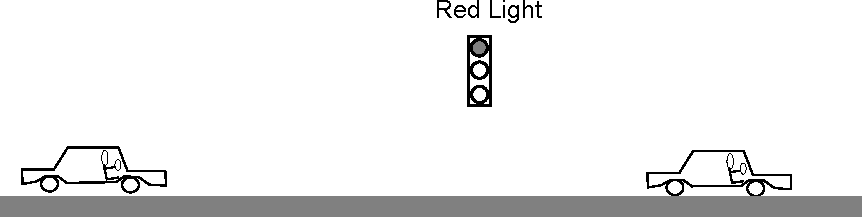
\includegraphics[width=0.8\textwidth]{images/03_red-light-speeding-slowing}
\end{center}
%
Now \underline{choose an $x$ axis} along the road by drawing an $x$-$y$ axis (your {\em choices} are: the position of the origin, and the positive $x$ direction). Then \underline{state whether each vector corresponds to a positive} \underline{or negative} one-dimensional value (you can just draw a ``($+$)'' or ``($-$)'' next to each). 

\subsection{Dynamics: Newton's Law(s)}

In 1687, Isaac Newton (English mathematician and physicist) published ``The Principia\footnote{It was written in Latin and the full title was: {\em  Philosophiæ Naturalis Principia Mathematica} (Mathematical Principles of Natural Philosophy).},'' which revolutionized human understanding of motion and its causes.  Prior to Newton, it was believed that the physical law proposed by Aristotle (Greek, 384--322 BCE) explained motion, essentially: {\em Objects move when pushed,  and stop moving when no longer pushed} \footnote{This might seem like a good law based on your own observations of the world (you're not alone: it held for 2000 years!). But it turns out that it is simply a good law for motion in a frictional fluid, like air.  If you add friction to Newton's correct description of motion, you obtain Aristotle's principle.}.  Following in the footsteps of Copernicus and Galileo, Newton proposed a better law of motion ({\bf Newton's Second Law}):
	%
	\begin{equation*}
	\textit{Objects change their motion when pushed} \quad\quad \text{or} \quad\quad \sum \vec{F} = m \vec{a} \quad \text{or} \quad\quad \vec{a} = \frac{\sum \vec{F}}{m}
	\end{equation*}
	%
where $\vec{F}$ is a {\bf force} (e.g., a push or pull interaction), the notation $\sum \vec{F}$ means ``the sum of all forces on the object'', and $m$ is the {\bf mass} of the object (e.g., in kilograms).  So Newton discovered that interaction {\em forces cause changes in velocity}.  Put another way: if there are no forces acting ($\sum \vec{F} = 0$) then there is no change to the velocity --- the object continues to move with the same velocity (vector).

Go back up to the two accelerating car(s) at the stoplight.  \underline{Draw a third vector} for each car called ``$\vec{F}$'' to indicate the force direction on the car that is causing its acceleration.  \underline{What do you think is causing} \underline{that force on the car(s)?}  (What is the {\em object} exerting the force?)

\vspace{0.5cm}

\subsection{Energy: Mechanical Energy}

The origin of the concept of energy in physics is through a quantity called {\bf Work}:
	%
	\begin{quote}
	Work is the energy transferred to an object by a force, found as {\em force times distance traveled}.
	\end{quote}
	%
or, as an equation:
	%
	\begin{equation*}
	W = F \Delta x  = \text{ Force} \times \text{distance } \quad \text{(positive when $\vec{F} \parallel \Delta \vec{x}$, negative when opposite)}
	\end{equation*}
	%
The connection of work to motion is that work causes changes in velocity.  Specifically, it changes what is called {\bf kinetic energy} of an object:
	%
	\begin{equation}
	K = \frac{1}{2} m v^2 	\quad \quad  \text{(Kinetic Energy, motional energy)}
	\end{equation}
	%
by the {\bf ``Work-Energy Theorem''}:
	%
	\begin{quote}
	The total work on an object is equal to the change in its kinetic energy: $W = \Delta K$.
	\end{quote}
	%
Another type of mechanical energy is {\bf Potential Energy}, which is stored energy (the potential to do work and cause kinetic energy). Common examples are springs (compressing an object against a spring) and gravity (raising an object up); in each case, ``releasing'' the object will allow the stored energy to be converted into motional kinetic energy.

For mechanical systems that have no friction, energy is always {\em conserved}: it can change from kinetic to potential, but will not be lost or gained.

\subsection{Energy: Other Energy}

Materials constructed from atoms (either the free-flowing fluids of liquids and gases, or the rigid lattices of solids) contain {\bf internal energy}.  If we think of these systems as just collections of little particles, then: (i)  a fluid's internal energy is determined by sum of the kinetic energy of all particles bouncing around in the container; (ii) a solid's internal energy is contained in the kinetic energy of the vibrating particles, and in the potential energy of the ``springs'' that connect them together.  When the number of particles in a material becomes very large, we treat the object as a thermal system: the {\em temperature} is a measure of the average internal energy of the particles.

There are other types of energy, some of which we will consider later: energy from electromagnetic radiation (light), electrical currents, nuclear energy.

\subsection{Energy: Equilibrium}

For an object that is both receiving enegy and giving away energy, we say that the object is in {\bf equilibrium} when:
	%
	\begin{quote}
	Rate of Energy In $=$ Rate of Energy Out  \hspace{1cm} (Equilibrium)
	\end{quote}
	

\section{Experiments and Activities}


\subsection{Motion}

Find a ``frictionless'' track and car and bring it to your lab bench.  Set it up and make sure that it is level by adjusting the ``feet.''  In each of these two experiments
	%
	\begin{enumerate}
	\item On a level track, give the car a kick at one end, and have your partner stop the car before it reaches the other end.
	\item Raise one end of the track and give the car a kick (not enough to go off the other end), then catch it.
	\end{enumerate}
	%
	perform the following tasks:
	%
	\begin{itemize}
	\item Do the experiment with the car (be sure to catch it before it reaches the ends).
	\item Time the experiment to get a range of times for your experiment.
	\item Observe the motion of the car during the whole time.
	\item Plot a position ($x$) vs time graph, and a velocity ($v$) vs time graph below it, as we did in lecture.
	\item Identify on the graph any time periods where the car is {\em accelerating}.  (How can you tell?)
	\end{itemize}
	%

\subsection{Mechanical Work}

Attach a pulley to the end of your track. Cut a long (3~m) piece of string and attach it to the car and to a mass-hanger with some amount of weight.
	%
	\begin{itemize}
	\item Record the amount of mass on your mass hanger (including the hanger itself).  Calculate the {\em weight}\footnote{The Weight of an object is the force of gravity on the object, $W = F_g = m g$, where $m$ is the mass in kilograms, $g$ is the ``acceleration due to gravity'' (10 m/$s^2$). The units on this product, kilograms times meters per second squared, are called {\em Newtons}, N.} of this amount using $\text{weight} = F_g = mg$.
	\item Do a few trials where you release the mass hanger from just below the table, letting it pull the car.
	\item Construct the position and velocity graphs again for this motion.
	\item Describe how this experiment relates to {\em work} and the {\em ``work energy theorem''}.
	\end{itemize}
	%
Return the track, the car, and the pulleys back to their places.

\subsection{Work and thermal energy}

Complete this with your whole table (4 people): one pair doing the stirring and one doing the hand-heating.
	%
	\begin{itemize}
	\item At the sink, fill up a glass beaker with cold water.  
	\item Then fill the two 50~mL graduated cylinders with the same water, to the same level (approximately 20~mL).  Record the level and the temperature.
	\item One pair will attempt to increase the temperature of the water by {\em mechanical work} (stirring with the plastic rod).
	\item The other pair will attempt to increase the temperature of the water by conduction with your hand.
	\item Conduct the experiment at least once for two minutes and record any temperature changes.
	\end{itemize}

\subsection{Equilibrium: Leaky Buckets}

Over the next few weeks in class, we will consider the energy equilibrium of the Earth, meaning the balance between the incoming energy per second from the Sun and the outgoing energy per second that the Earth emits into space.  In turns out that, while the incoming rate (energy from the sun) is approximately unchanging, the outgoing rate {\em depends on the Earth's temperature}.   As an equation, it looks like this:
	%
	\begin{equation*}
	Rate_\text{  Sun Energy In} = Rate_\text{  Earth Energy Out} \left(T_\text{Earth} \right)
	\end{equation*}
	%
where the parentheses on the right-hand side means that the rate {\em depends} on temperature.  The importance of this dependence is that in a situation of equilibrium (when the left-hand side equals the right-hand side) the result implies a single temperature: we can determine the temperature of the Earth by assuming equilibrium.

Today we will play with an analogy of this situation: a ``leaky bucket'' that is being filled by a variable-rate pitcher.  We will see if the equilibrium flow rate depends on any properties of the system (like the rate of energy into/out-of the Earth depends on its temperature).

\vspace{1cm}

\noindent Complete the following, using the data table on the next page, and eventually making a graph on graph paper of the last two columns.
	%
	\begin{itemize}
	\item Fill the pitcher of water about $3/4$ full.
	\item Raise the blue ``lab jack'' up so that the 100~mL graduated cylinder will fit underneath the pitcher spout.
	\item Place the catch tray below the spout and then connect the aquarium pump: the pump will be sitting on the table with one rubber tube (IN) going into the catch tray, and another rubber tube (OUT) going into the pitcher.  You can test that this is working by plugging in the pump and letting the water flow from the pitcher into the catch tray, and back to the pitcher through the pump.
	\item Place the 100~mL graduated cylinder (GC) in the catch tray and let the water go out of the spout into the cylinder.  Record any general observations.
	\item Now adjust the flow from the spout so that the level of the water in the GC is just a little bit above the hole (couple mL).  
	\item On the table, record the {\em baseline} level (the value on the GC of the center of the hole).
	\item In ``Approx Level'' put ``just above hole'', and record its ``Exact Level'', and then subtract off the baseline value to get the $\Delta V$ value.
	\item Now remove the GC without changing the flow.
	\item Use the 25~mL graduated cylinder and the stopwatch to time how long it takes to fill (to the 25~mL line).  Record this in your table under ``Time to 25~mL''.  It would be best to do this three times, take the average and record the average and approximate uncertainty. You can then calculate the  ``Flow Rate'' (or you can wait to do that later for all of the data you collect).
	\item In the rest of the rows of the table, choose successively larger flow rates. The ``Approx level'' could give you a target to try and find (like ``twice the $\Delta V$ as the first'', or three times, etc), but always record the exact level that you have.
	\item In the end calculate the height in cm from the $\Delta V$ column by measuring the distance on the GC itself.  
	\item On graph paper, make a plot of your data: either Flow rate vs Height, or vice-versa\footnote{When we say ``y vs x'' we mean ``vertical vs horizontal''.}.
	\end{itemize}


\newpage
%%%%%%%%%%%%%%%%     DATA TABLE         %%%%%%%%%%%%%%%%%%%%%%%%
\renewcommand{\arraystretch}{1.4}

\begin{center}
\begin{tabular}{|p{2.5cm}|p{2.5cm}|p{2.5cm}|p{2.5cm}|p{2.5cm}|p{2.5cm}|}
\hline
\textbf{Approx level} &
\textbf{Exact Level} &
\textbf{$\Delta V$}\newline (above hole) &
\textbf{Time to \newline25 mL} &
\textbf{Flow Rate} &
\textbf{Height} \\
\hline
 (  \hspace{1cm} )  & (  \hspace{1cm} )  &(  \hspace{1cm} ) & (  \hspace{1cm} ) & (  \hspace{1cm} )  & (  \hspace{1cm} )  \\   % units row
\hline
\hline
Baseline Value (Hole Center) &  &  \cellcolor{gray!90}  &  \cellcolor{gray!90} &  \cellcolor{gray!90}   &  \cellcolor{gray!90}  \\[1.5em]
\hline
 & & & & & \\[1.5em]
\hline
 & & & & & \\[1.5em]
\hline
 & & & & & \\[1.5em]
\hline
 & & & & & \\[1.5em]
\hline
 & & & & & \\[1.5em]
\hline
 & & & & & \\[1.5em]
\hline
 & & & & & \\[1.5em]
\hline
 & & & & & \\[1.5em]
\hline
 & & & & & \\[1.5em]
\hline
\end{tabular}
\end{center}
Be sure to fill in the units in the second row.








 